\chapter{Laporan}
\section{PEMAHAMAN TEORI}
\subsection{FUNGSI}
\begin{enumerate}
	\item Fungsi adalah salah satu blok program yang sudah terorganisir terdiri dari nama fungsi, input variabel dan variabel kembalian. Fungsi digunakan untuk aplikasi anda dan tingkat penggunaan kode yang tinggi agar aplikasi lebih baik.
	\item inputan fungsi digunakan untuk menerima baris input dari user dan mengembalikannya dalam bentuk string.
	\item kembalian fungsi yaitu fungsi akan membaca sebaris input umumnya melalui keyboard sampai nanti dijumpai karakter newline(enter) dan akan mengembalikan string dari inputan tersebut.  
\end{enumerate}
\lstinputlisting[language=Python]{src/KodingTeori1.py}

\subsection{PAKET}
\begin{enumerate}
\item Paket adalah sebuah manifestasi dari konsep namespace hierarkis python.
\item cara pemanggilan paket  
\lstinputlisting[language=Python]{src/KodingTeori2.py}
\end{enumerate}

\subsection{KELAS}
\begin{enumerate}
\item kelas adalah prototipe yang ditentukan oleh pengguna untuk objek yang mendefinisikan seperangkat atribut yang menjadi ciri khas dari sebuah kelas apa pun. Class digunakan untuk membuat kelas baru dan nama kelas diikuti kanca kunci titik dua. 
\item Objek adalah perwujudan dari sebuah class. Bila kelas adalah prototipe nya, dan objek adalah barang jadinya. 
\item atribut yaitu semua class yang membuat objek dan semua objek tersebut mengandung karakteristik.
\item method merupakan fungsi yang didefinisikan di dalam suatu class.
\end{enumerate}
\lstinputlisting[language=Python]{src/KodingTeori3.py}
\subsection{Cara pemanggilan library kelas dari instansiasi dan pemakaiannya contoh dengan program}
untuk membuat objek dari sebuah kelas, kita memanggil nama kelas dengan argumen yang sesuai dengan   fungs pada saat kita mendefinisikannya.
\\cara pemanggilan\\
\lstinputlisting[language=Python]{src/KodingTeori4.py}
\subsection{Pemakaian paket dengan perintah from kalkulator import penambahan}
Pertama-tama kalian harus membuat program kalkulator.py untuk bisa melakukan penambahan sperti di bawah
\lstinputlisting[language=Python]{src/KodingTeori5.py}
\subsection{Pemakaian paket fungsi apabila file library ada di dalam folder}
Untuk pemakaian paket fungsi apabila file library berada di folder yaitu untuk dapat melakukan atau menjalankan kalkulator yang berada di file folder.
\lstinputlisting[language=Python]{src/KodingTeori6.py}
\subsection{Pemakaian paket kelas apabila file library ada di dalam folder}
Untuk pemakaian paket kelas apabila file library berada di folder.Mahasiswa yaitu file Mahasiswa untuk melakukan atau menjalankan kode yang berada di file folder Mahasiswa tersebut.
\lstinputlisting[language=Python]{src/KodingTeori7.py}
\section{KETERAMPILAN PEMROGAMAN}
\lstinputlisting[language=Python]{src/NPM1.py}
\lstinputlisting[language=Python]{src/NPM2.py}
\lstinputlisting[language=Python]{src/NPM3.py}
\lstinputlisting[language=Python]{src/NPM4.py}
\lstinputlisting[language=Python]{src/NPM5.py}
\lstinputlisting[language=Python]{src/NPM6.py}
\lstinputlisting[language=Python]{src/NPM7.py}
\lstinputlisting[language=Python]{src/NPM8.py}
\lstinputlisting[language=Python]{src/NPM9.py}
\lstinputlisting[language=Python]{src/NPM10.py}
\lstinputlisting[language=Python]{src/kalkulator.py}
\lstinputlisting[language=Python]{src/Mahasiswa.py}
\lstinputlisting[language=Python]{src/Ngitung.py}
\lstinputlisting[language=Python]{src/3lib.py}
\lstinputlisting[language=Python]{src/main.py}
\lstinputlisting[language=Python]{src/kelas3lib.py}
\lstinputlisting[language=Python]{src/main.py}
\section{KETERAMPILAN PENANGANAN ERROR}
\lstinputlisting[language=Python]{src/KeterampilanPenangananError.py}
\section{LAMPIRAN PLAGIARISM}
\begin{figure}[H]
		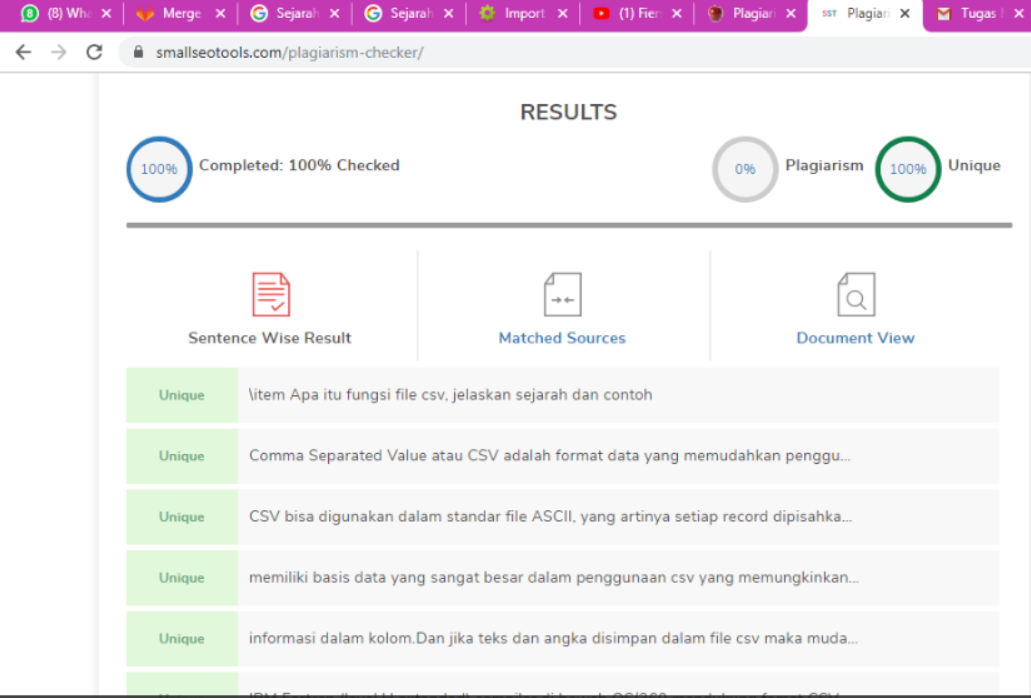
\includegraphics[width=4cm]{figures/1184065/ss1.PNG}
		\centering
		\caption{Screnshoot Plagiarism}
	\end{figure}
	\begin{figure}[H]
		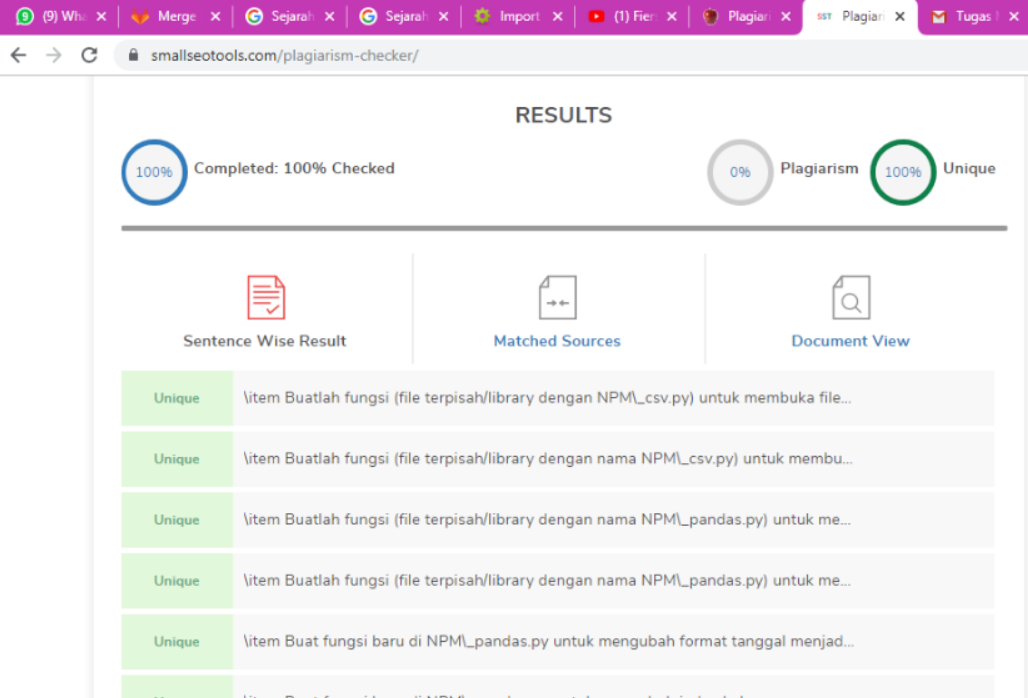
\includegraphics[width=4cm]{figures/1184065/ss2.PNG}
		\centering
		\caption{Screnshoot Plagiarism}
	\end{figure}
\section{LINK YOUTUBE}
\begin{enumerate}
\item \href{https://youtu.be/FDE8KrHC4m4}{klik}
\item \href{https://youtu.be/qzmEN1LVhsM}{klik}
\item \href{https://youtu.be/3UKVrJmwmYo}{klik}
\item \href{https://youtu.be/3UKVrJmwmYo}{klik}
\end{enumerate}







